\section{Introduction}

Heegaard Floer homology is an invariant of 3-manifolds introduced by Ozsv\'{a}th and Szab\'{o} \cite{OzsvathSzabo}. In its simplest form, it associates to a closed 3-manifold $Y$ a graded $\mathbb{F}_2$ vector space, denoted $\widehat{HF}(Y)$. It was shown by Ozsv\'{a}th and Szab\'{o} \cite[Proposition 5.1]{OS2} that if $Y$ is a rational homology 3-sphere then
\begin{align*}
\textup{rk }\widehat{HF}(Y)\geq{}|H_1(Y ; \mathbb{Z})|.
\end{align*}

\begin{definition}An \emph{L-space} is a rational homology sphere $Y$ with simplest possible Heegaard Floer homology, that is, with
\begin{align*}
\textup{rk } \widehat{HF}(Y) = |H_1(Y ; \mathbb{Z})|.
\end{align*}
\end{definition}

Lens spaces are L-spaces, motivating the name. It is interesting to ask whether there exist alternative characterizations of L-spaces that do not depend on Heegaard Floer homology \cite[Question 11]{OS4}. We know that if $Y$ is an L-space then $Y$ does not admit a $C^{2}$ co-orientable, taut foliation \cite{OS3}. The non-existence of a co-orientable, taut foliation has been proposed by Ozsv\'{a}th and Szab\'{o} as a possible characterization of L-spaces. Along similar lines, a conjecture has been proposed \cite{BoyerGordonWatson} that attempts to characterize L-spaces through a property of their fundamental group.

\begin{conjecture_main}
An irreducible rational homology 3-sphere is an L-space if and only if its fundamental group is not left-orderable.
\end{conjecture_main}

Recall that a left-orderable group is a group which admits a left-invariant total order.

The conjectured relationship between L-spaces and left-orderability is already known for 3-manifolds that are double branched covers of non-split alternating links. It has been shown that for a non-split alternating link $K\subset S^3$, the fundamental group of $\Sigma{}(K)$ is not left-orderable \cite{BoyerGordonWatson} (cf. \cite{GreeneJE}, \cite{Ito}), where $\Sigma{}(K)$ denotes the double branched cover of $K\subset{}S^3$. Furthermore, Manolescu and Ozsv\'{a}th \cite{ManolescuOzsvath} showed that alternating links, and more generally, quasi-alternating knots, are homologically thin. In turn, Ozsv\'{a}th and Szab\'{o} showed in \cite{OzsvathandSzabo} that for a homologically thin link $K$, its double branched cover is an L-space. Therefore, if a 3-manifold $M$ is the double branched cover of some non-split alternating link, then $M$ is an L-space and $\pi_1(M)$ is not left-orderable.

We will verify that a specific class of L-spaces arising from the double branched covers of Kanenobu's knot (see Figure~\ref{figure:kanenobu}) have fundamental groups which are not left-orderable. We will consider the knots $K_n$ for $n\geq{}0$, defined as
\begin{align*}
K_n=K_{-10n,10n+3}.
\end{align*}
\noindent{}It was shown by Greene and Watson that $K_n$ is homologically thin (but not quasi-alternating), and so $\Sigma{}(K_n)$ is an L-space for $n\geq{}0$ \cite[Proposition 11]{GreeneWatson}. Generically, $K_n$ is non-alternating and $\Sigma{}(K_n)$ is hyperbolic and can not be obtained by surgery on a knot in $S^{3}$ \cite{HoffmanWalsh}, so these manifolds fall outside of the classes considered in \cite{BoyerGordonWatson}. The fundamental group, $G_n$, of the double branched cover of $K_n$ was computed by Greene and Watson \cite{GreeneWatson}, and has the following presentation:


\begin{align*}
G_n=\pi{}_1(\Sigma{}(K_n))=\langle a,\; b,\; c,\; d \mid{} &(a^{-1}b)^{10n}d^{-1}a^{2},\; b^{-2}c(b^{-1}a)^{10n},\\
&(d^{-1}c)^{10n+3}c^{-1}bc^{-2},\; d^{2}a^{-1}d(c^{-1}d)^{10n+3} \rangle
\end{align*}
where we have renamed the four generators $v_1$, $v_2$, $v_3$, and $v_4$ from the original paper as $a$, $b$, $c$, and $d$, respectively.

\begin{figure}[ht]
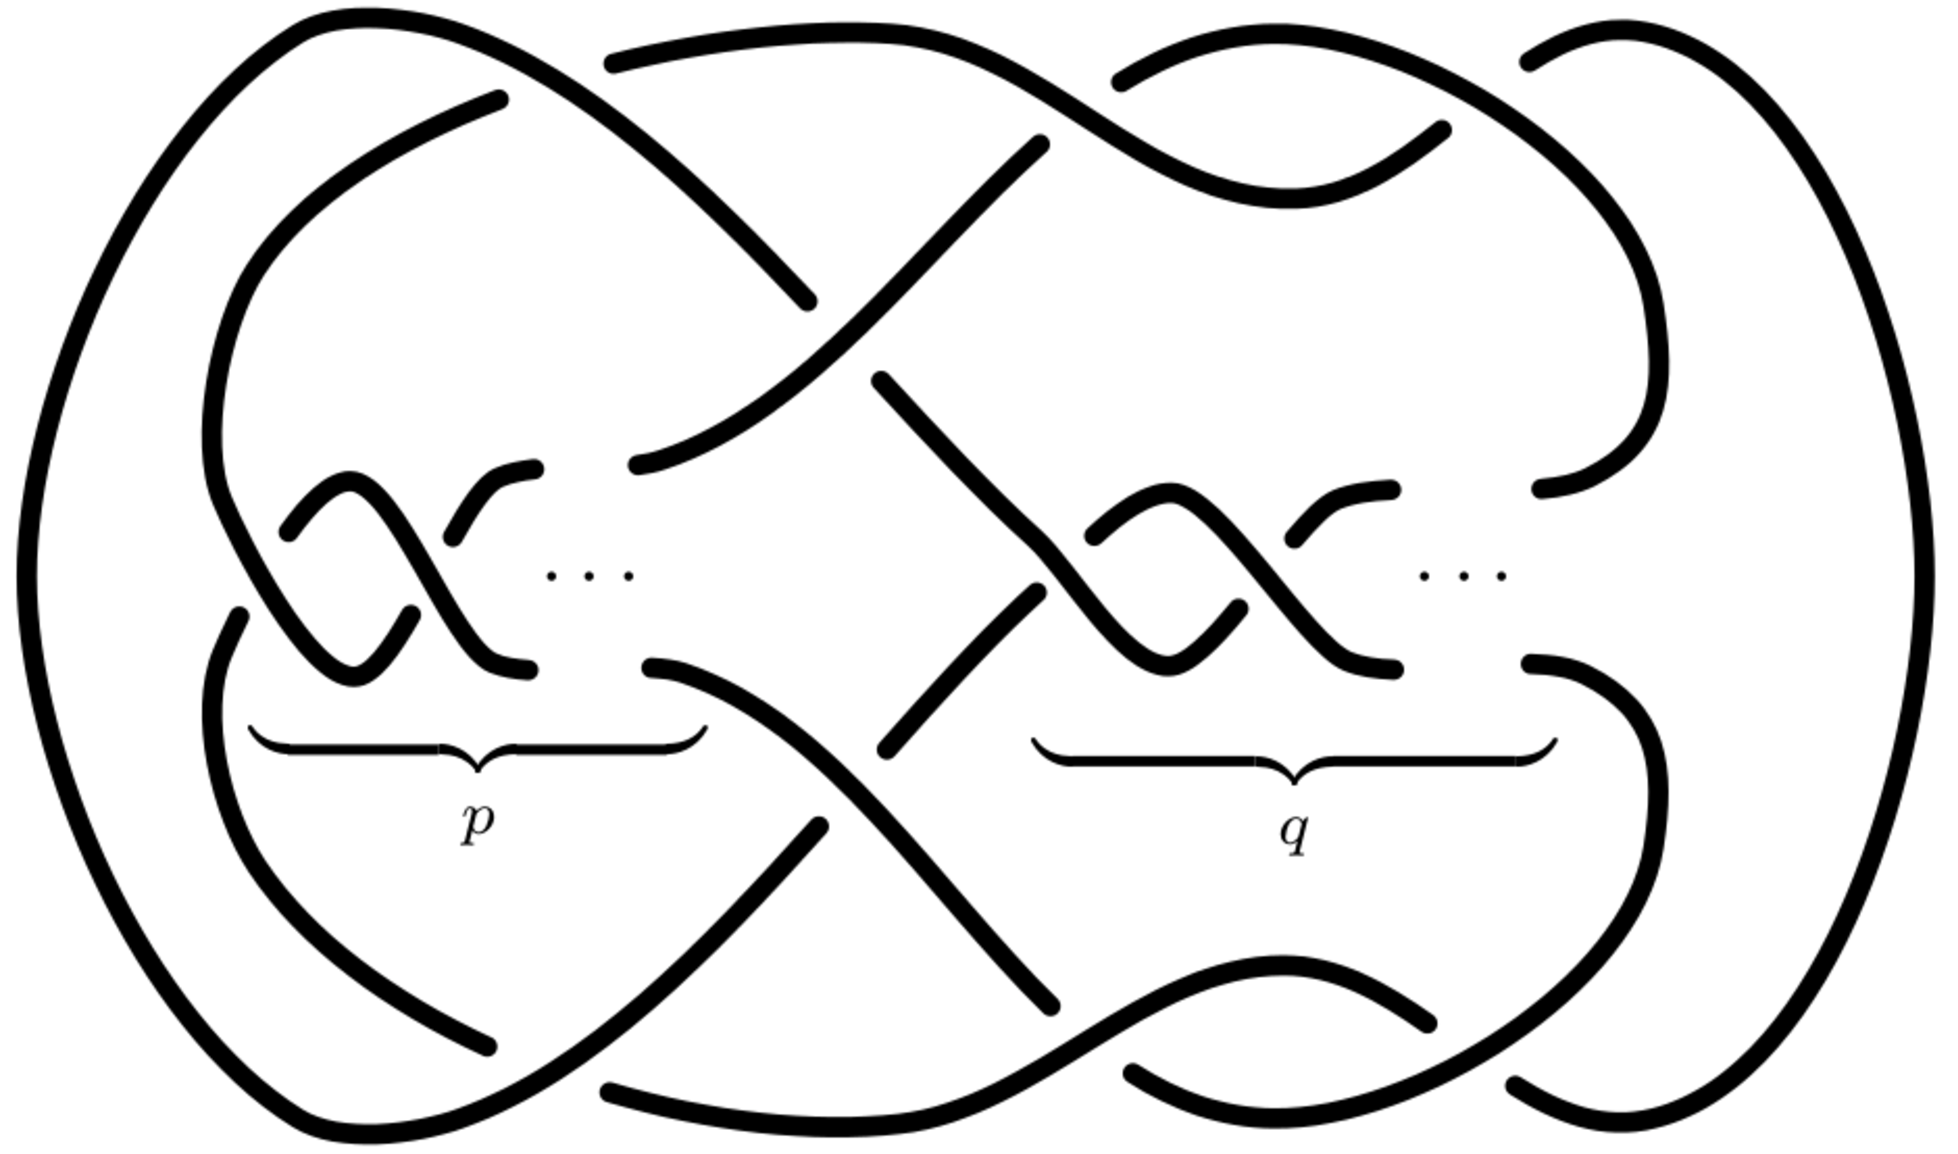
\includegraphics[scale=.37]{kanenobu}
\caption{Kanenobu's knot $K_{p,q}$. Image due to \cite{GreeneWatson}.}
\label{figure:kanenobu}
\end{figure}

\begin{theorem*} The fundamental group $G_n$ of the double branched cover of $K_n$ is not left-orderable.
\label{MAINTHEOREM}
\end{theorem*}

\noindent{} Next, we introduce various definitions and give background on left-orderability.

\subsection{Left-orderability}

%\begin{definition}

%A {\it total order} on a set $X$ is a binary relation $\leq$ satisfying the following for all $x, y, z \in{} X$:
%\begin{enumerate}
%\item $x\leq{}x$ (reflexivity)
%\item $x\leq{}y$ and $y\leq{}x$ implies $x=y$ (anti-symmetry)
%\item $x\leq{}y$ and $y\leq{}z$ implies $x\leq{}z$ (transitivity)
%\item $x\leq{}y$ or $y\leq{}x$ (totality)
%\end{enumerate}
%\end{definition}

\begin{definition}
A group $G$ is {\it left-orderable} if its elements can be given a left-invariant total order. That is, a total order $<$ such that $g<h$ implies $fg<fh$ for all $f, g, h\in{}G$.
\end{definition}

\begin{remark} By convention the trivial group is not left-orderable.
\end{remark}

%\begin{definition} Given a left-orderable group $(G,<)$ we can define a %binary relation $<$ on $G$ in the following way:
%\begin{align*}
%x<y\Leftrightarrow{}x\leq{}y\; \textrm{and} \; x\neq{}y.
%\end{align*}
%\end{definition}
We recall some facts on left-orderable groups from \cite{ClayRolfsen}.

\begin{fact} For some left-orderable group $(G, <)$ we can define {\it a} corresponding relation $>$ in the following way: for $g,h\in{}G$, $g>h$ if and only if $h<g$. This notational convenience will be used frequently.
\end{fact}

\begin{fact} In a left-orderable group G, $1<g$ (``$g$ is positive") if and only if $g^{-1}<1$ (``$g^{-1}$ is negative").
\label{fact:inverses}
\end{fact}
%\begin{proof}
%\begin{align*}
%1<g\Leftrightarrow{}(g^{-1})1<(g^{-1})g\Leftrightarrow{}g^{-1}<1.
%\end{align*}
%\end{proof}

\begin{fact} Transitivity implies that in a left-orderable group products of positive elements are positive and products of negative elements are negative.
\label{1.3LO}
\end{fact}

%\noindent{}We now prove a few useful properties of left-orderable groups.
\begin{proposition} In a left-orderable group $G$, $g\in{}G$ has the same sign as $g^{n}$ for any $n>1$.
\label{proposition:pospowers}
\end{proposition}
\begin{proof} Consequence of Fact \ref{1.3LO}.
%The claim is clear if $g=1$, so we can assume $g<1$. Note that if $g>1$, then we can multiply both sides on the left by $g$ to obtain $g^2>g>1$ and once more to obtain $g^3>g^2>g>1$. Continuing this process shows that $g^n>1$ for any $n>1$ if $g>1$. Similarly, $xg^n<1$ for any $n>1$ if $g<1$. Suppose now that $g>1$ and suppose (for contradiction) that $g^{n}<1$ for some $n>1$. By Proposition~\ref{proposition:inverses}, $g^{-1}<1$ and as noted above, this shows that $g^{n-1}<1$ for any $n>1$. Therefore, $g=(g^{n-1})(g^n)<g^{n-1}<1$, contradicting the fact that $g>1$. A similar proof works when $g<1$.
\end{proof}

\begin{fact} A left-orderable group has no torsion.
\label{fact:torsion}
\end{fact}
%\begin{proof} Suppose G is a left-orderable group, and suppose (for contradiction) that there exists some non-trivial $g\in{}G$ such that $g^{n}=1$ for some $n>1$. We know that either $g>1$ or $g<1$. If $g>1$ then $g^{2}>g>1$ and $g^{3}>g^{2}>g>1$. We can continue this process until we reach $g^{n}$:
%\begin{align*}
%1=g^{n}>g^{n-1}>\cdots{}>g^{2}>g>1.
%\end{align*}
%This is a contradiction. The case when $g<1$ is similar.
%\end{proof}

%\begin{corollary} Every finite group is not left-orderable.
%\end{corollary}
%\begin{proof} Suppose $G$ is a group of finite order. Note: by convention, the trivial group is not left-orderable. We will assume $G$ is non-trivial. Choose $g\in{}G$ such that $g\neq{}1$. The cyclic subgroup $\langle{}g\rangle{}\subset{}G$ is necessarily finite since it is a subgroup of the finite group $G$. This means that $g^{n}=1$ for some $n>1$, and thus $G$ is not left-orderable by Fact~\ref{fact:torsion}.
%\end{proof}

\begin{fact} Let $G$ be a non-trivial group and let $g\in{}G$. There exists a left-ordering $<$ on $G$ such that $g<1$ if and only if there exists a left-ordering $<^\prime$ on $G$ such that $1<^\prime g$.
\label{fact:WLOG}
\end{fact}
%\begin{proof} Suppose there exists a left-ordering $<$ on $G$ such that $g<1$. For $x,y\in{}G$, define $<'$ by:
%\begin{align*}
%x<'y\Leftrightarrow{}y<x.
%\end{align*}
%Because of the properties of $<$, $<'$ is clearly a left-invariant total ordering on $G$. With this definition of $<'$, it is clear that $1<'g$. A similar proof is clear for the converse direction.
%\end{proof}

\noindent{}We can also define left-orderability in a different way:

\begin{proposition} A group $G$ is left-orderable if and only if there exists a subset $P\subset{}G$ such that:
\begin{enumerate}
\item $P\cdot{}P\subset{}P$
\item $P\cap{}P^{-1}=\emptyset{}$
\item $G=P\cup{}P^{-1}\cup{}\{ 1 \}$
\end{enumerate}
\label{proposition:poscone}
\end{proposition}
\begin{proof} Suppose $G$ is left-orderable. Define
\begin{align*}
P=\Set*{g\in{}G}{1<g}.
\end{align*}
Then $P\cdot{}P\subset{}P$ since if $g>1$ and $h>1$ then $gh>g>1$. Therefore, $P$ satisfies the first condition. If $g>1$ then $g^{-1}<1$ and so $P\cap{}P^{-1}=\emptyset{}$. Therefore, $P$ satisfies the second condition. Finally, by the totality of a total ordering, all non-trivial elements in $G$ must be either positive or negative, thus $P\cup{}P^{-1}\cup{}\{ 1 \}$. Therefore, $P$ satisfies the third condition, completing one direction of the proof.\\
\\
Conversely, suppose there exists a subset $P\subset{}G$ satisfying the three conditions of the proposition. Define a left ordering in the following way:
\begin{align*}
g<h\Leftrightarrow{}g^{-1}h\in{}P.
\end{align*}
It is easy to check this defines a left-ordering.
%We will now verify that this is a left-invariant total order. Reflexivity is clear. Anti-symmetry follows from the second condition on $P$, namely  $P\cap{}P^{-1}=\emptyset{}$. This means that it is not possible for both an element and its inverse to be in $P$, and thus for $x,y\in{}G$, $x<y$ and $y<x$ is impossible, so $x\leq{}y$ and $y\leq{}x$ implies $x=y$. Totality is clear from the fact that $G=P\cup{}P^{-1}\cup{}\{ 1 \}$. To prove transitivity, suppose $x,y,z\in{}G$ and $x<y$ and $y<z$. Then $x^{-1}y\in{}P$ and $y^{-1}z\in{}P$. Since $P\cdot{}P\subset{}P$, $(x^{-1}y)(y^{-1}z)=x^{-1}z\in{}P$, and thus $x<z$. Therefore, $<$ is a total order on $G$. Now for $g,h,x\in{}G$, suppose $g<h$. Then:
%\begin{align*}
%g^{-1}h\in{}P\\
%\Rightarrow{}g^{-1}(x^{-1}x)h\in{}P\\
%\Rightarrow{}(g^{-1}x^{-1})(xh)\in{}P\\
%\Rightarrow{}xg<xh.
%\end{align*}
%This shows that $<$ is a left invariant total order, completing the proof.
\end{proof}

\begin{definition} For a group $G$, a subset $P\subset{}G$ satisfying the three conditions of Proposition~\ref{proposition:poscone} is called a {\it positive cone}.
\end{definition}

%\subsection{Double Branch Cover}

%
%\begin{definition}
%A 3-manifold that can be obtained as a union of two solid tori associated by a homeomorphism of their boundaries is called a \emph{lens space}
%\end{definition}
%}

\subsection{Heegaard Floer Homology, L-Spaces, and Lens Spaces}
Heegard Floer homology is an invariant of 3-manifolds, introduced by Ozsv\'{a}th and Szab\'{o} \cite{OzsvathSzabo}. It associates a closed 3-manifold $Y$ a graded vector space over $\mathbb{F}_2$, denoted $\reallywidehat{HF}(Y)$.
\begin{definition}An \emph{L-space} is a rational homology sphere $Y$ with simplest possible Heegaard Floer homology, that is, with
\begin{align*}
rk \reallywidehat{HF}(Y) = |H_1(Y ; \mathbb{Z})|.
\end{align*}
All lens spaces have this property.
\end{definition}

%\subsection{Black and White Graphs, and Greene's Theorem}

%{\begin{definition} The {\it black and white graphs of a knot diagram}: $D\rightarrow{}R^{2}\setminus{}D$
%\label{DefBWD}
%\begin{enumerate}
%\item One vertex for each white/black region
%\item One edge for each crossing
%\item Sign convention for $\mu(x_i,x_j)$
%\begin{figure}[h]
%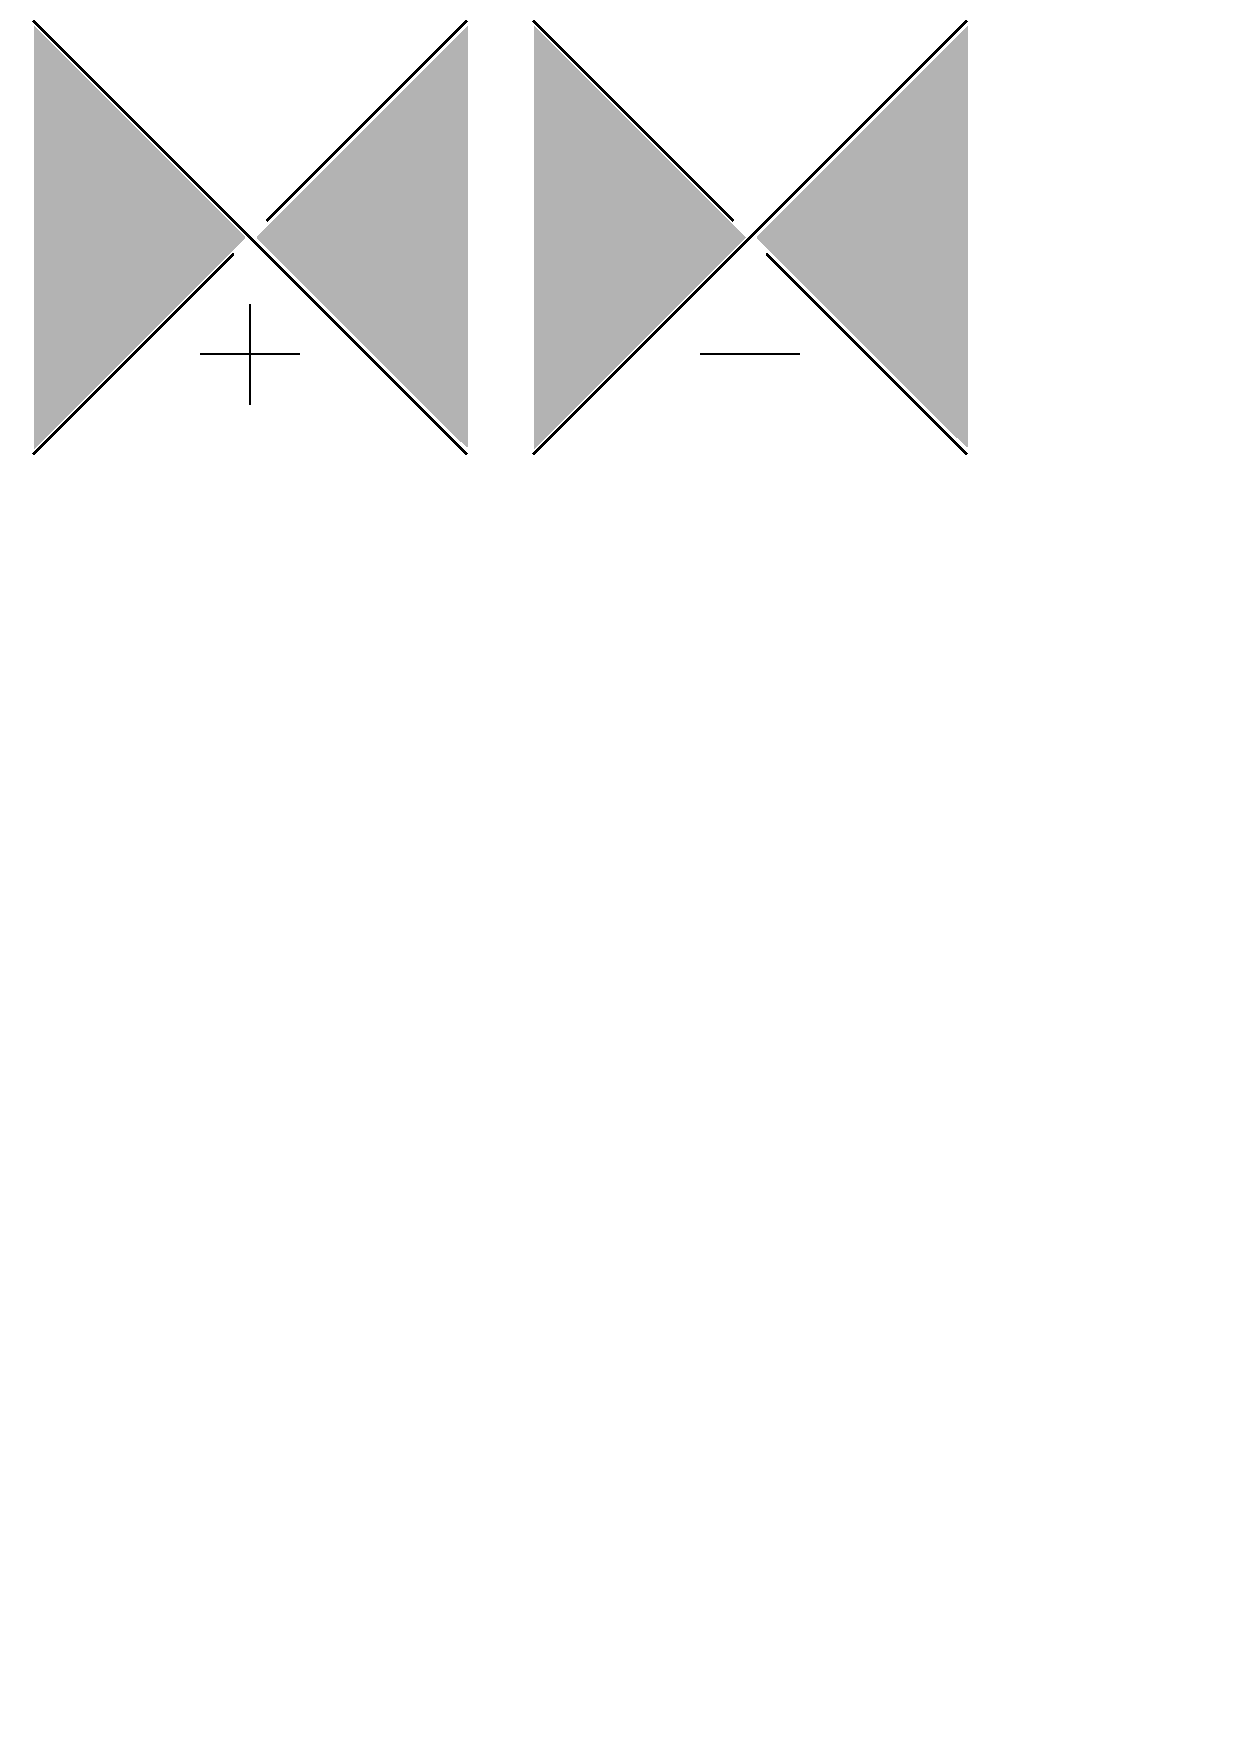
\includegraphics[scale=.37]{signconvention}
%\caption{$\mu(x_i,x_j)$: Sign conventions for the black and white graph.}
%\label{figure:MuCon}
%\end{figure}
%\end{enumerate}
%\end{definition}

%\begin{theorem_greene}
%\label{Greene}
%Let $\Sigma(K)$ denote the double branch cover of some knot K. Then%, and fix a white graph W for some diagram of K. Then $\pi_1(\Sigma(K))\cong{}G_W$:
%\begin{align*}
%\pi_1(\Sigma(K))=\langle{}x_1, x_2,..., x_n:r_1,r_2,...,r_n,x_r\rangle{}
%\end{align*}
%\begin{enumerate}
%\item $x_i$ is a vertex in the white graph of K
%\item $r_i$ is the relator assigned to a vertex
%\item $x_r$ is the root vertex of the white graph of K
%\end{enumerate}
%\begin{align*}
%r_i=(x_i^{-1}x_j)^{\mu(x_i,x_j)}...(x_i^{-1}x_k)^{\mu(x_i,x_k)}.
%\end{align*}
%\end{theorem_greene}

%\begin{figure}[h]
%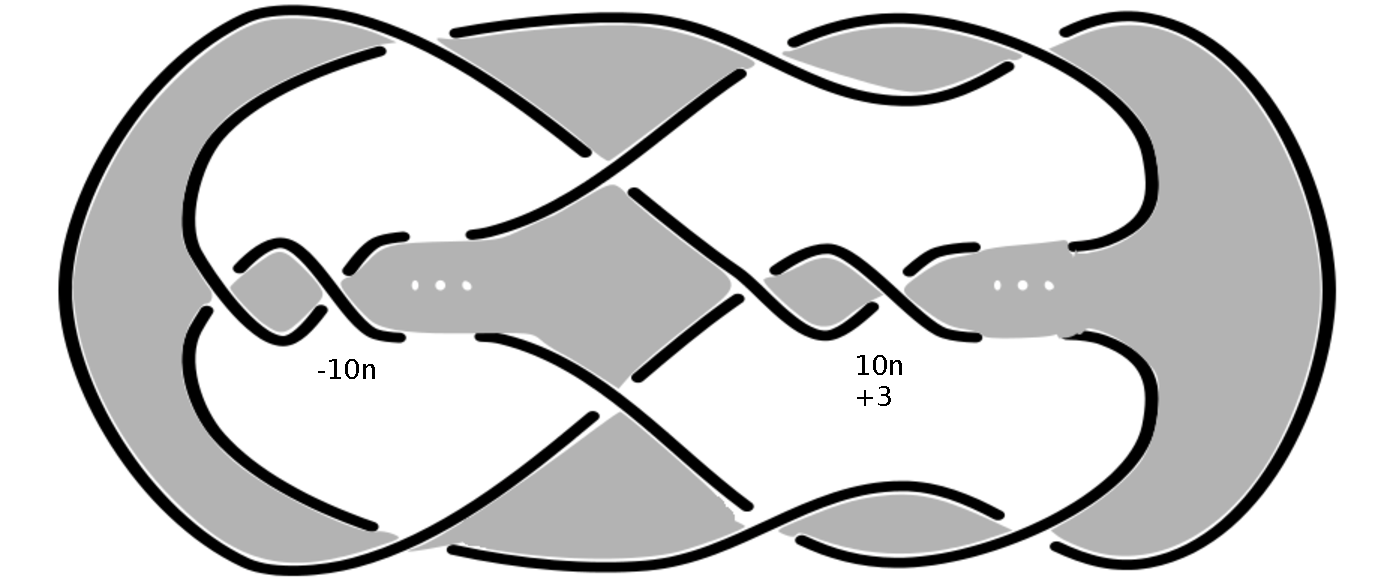
\includegraphics[scale=.5]{KanenobuBW}
%\caption{Checkerboard coloring of $K_{-10n,10n+3}$. Original image due to \cite{GreeneWatson}.}
%\label{figure:kanenobuCheckboard}
%\end{figure}

%\begin{figure}[h]
%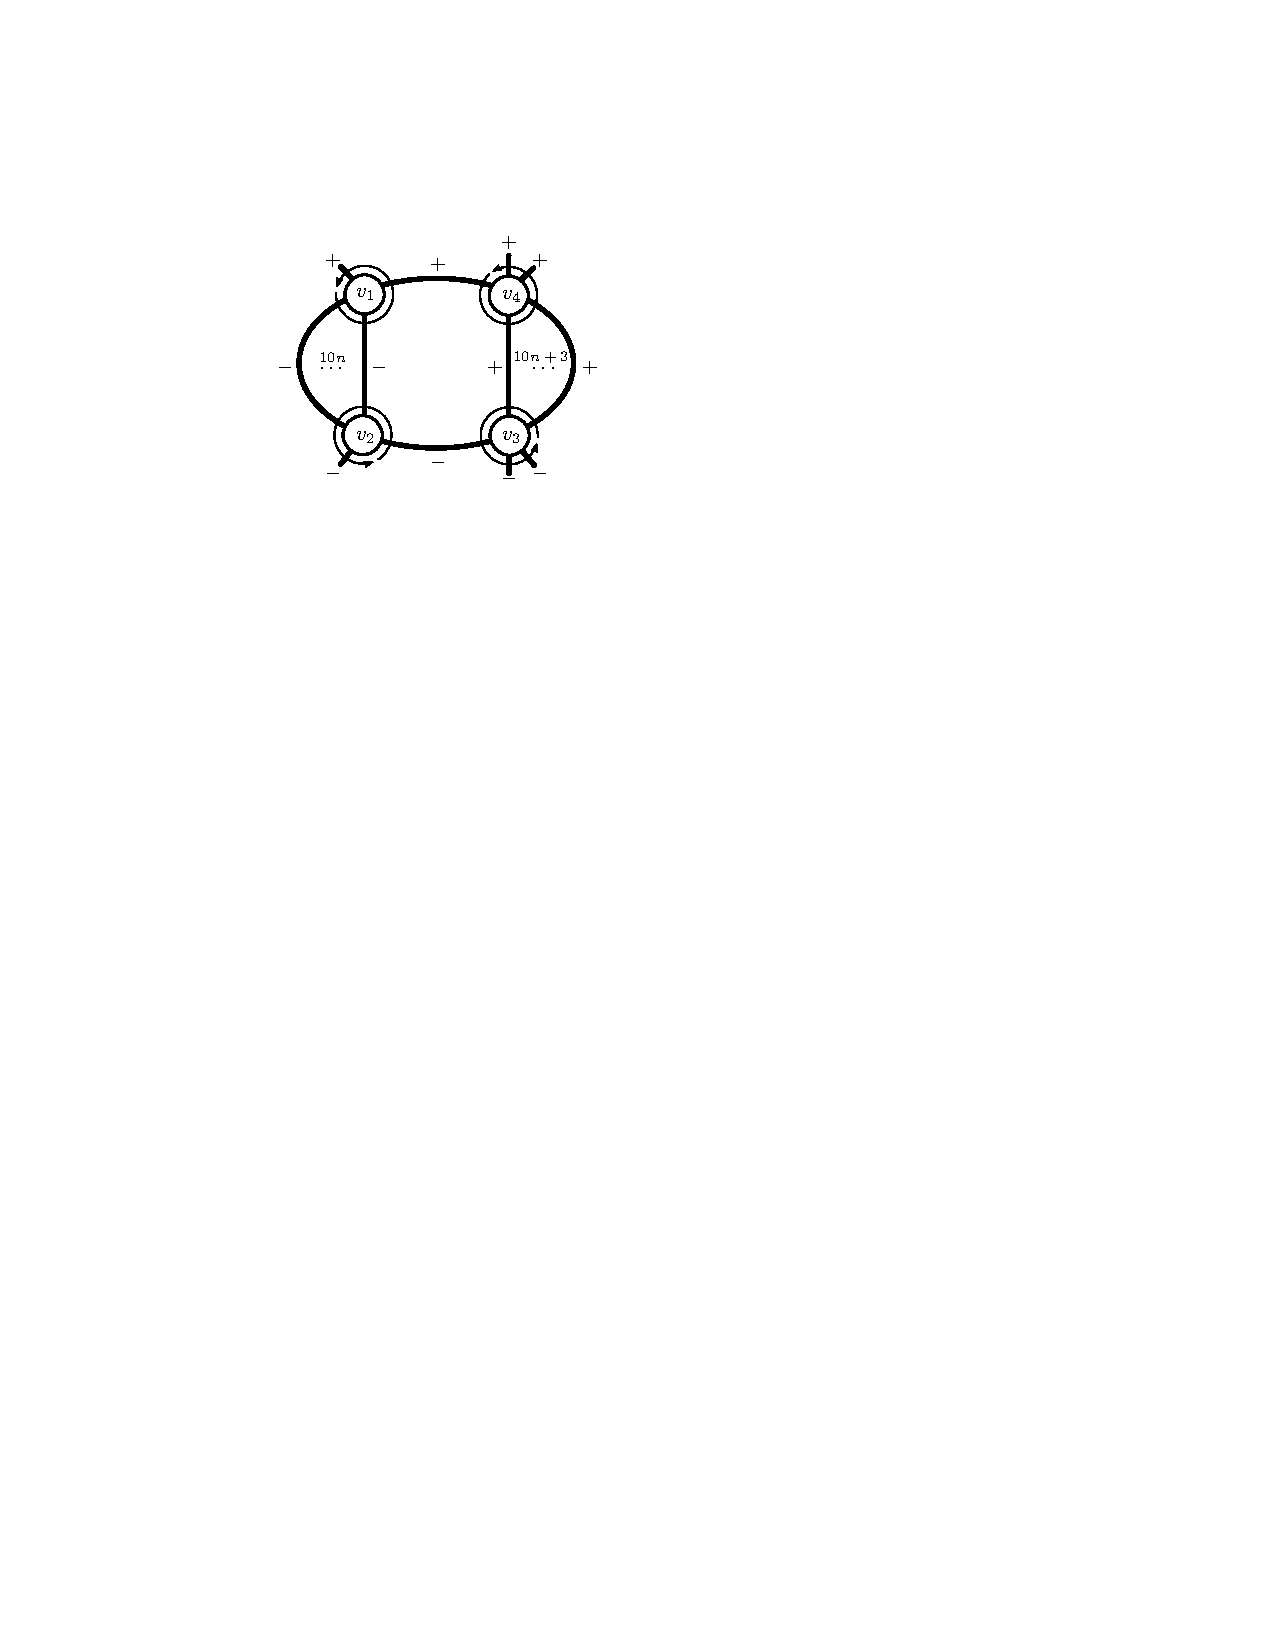
\includegraphics[scale=2]{KanenobuWG}
%\caption{White graph for $K_{-10n,10n+3}$. Note that edges which appear not to connect to any vertices actually connect to the root vertex, which is not shown. Image due to \cite{GreeneWatson}.}
%\label{figure:kanenobuWG}
%\end{figure}

%The checkerboard coloring of $K_n$ is shown in Figure~\ref{figure:kanenobuCheckboard}. Using this, and Following the procedures outlined in Definition~\ref{DefBWD}, we have Figure \ref{figure:kanenobuWG}, and by Greene's Theorem, we have that for all $n\geq{}0$ from

\subsection{Automated Proofs}
Several of the proofs for lemmas and propositions in this paper were generated by a computer program we created for the task. We will now briefly describe the algorithm our program employs, as it could be useful for future work in disproving the left-orderability of certain groups. Our program is similar to the program described in \cite[Section 8]{CalegariDunfield}.

For the proof that $G_n$ is not left-orderable, we argue by contradiction. That is, we assume that $G_n$ is left-orderable, thus for any left-ordering on $G_n$, there must exist a positive cone $P\subset{}G_n$. Based on Fact~\ref{fact:WLOG}, we can proceed under the assumption that $b^{-1}a\in{}P$, and then find additional elements of $G_n$ that must be contained in such a positive cone. With the addition of enough elements, we can in many cases reach a contradiction.

In order to accomplish this, the program takes two inputs:
\begin{enumerate}
\item A set $Q\subset{}P$ of elements that have been proven (either in previous iterations of the program, or by hand) to be contained in $P$, including $b^{-1}a$. This set will grow during the execution of the program, but we will ensure that it always is a subset of $P$, so $Q$ has the property inherited from $P$ that $1\not\in Q^{*}$, where $Q^*$ is the semigroup generated by $Q$. 
\item A subset $I$ of all words that we know are equal to the identity based on the group relations of $G_n$, closed under inversion and cyclic permutation. See (\ref{intro:cyclic}) for an example of what is meant by cyclic permutation.
\end{enumerate}
\begin{remark}
Words that are equal to the identity are henceforth referred to as identities.
\end{remark}
The four group relations of $G_n$ are obvious examples of identities. To give another example, Lemma~\ref{lemma:eq5} shows that $d^{-1}a^{2}b^{-2}c$ is also an identity. The cyclic permutations of this identity would be:
\begin{align}
\{d^{-1}a^{2}b^{-2}c,\; cd^{-1}a^{2}b^{-2},\; b^{-1}cd^{-1}a^{2}b^{-1},\nonumber{}\\
b^{-2}cd^{-1}a^{2},\; ab^{-2}cd^{-1}a,\; a^{2}b^{-2}cd^{-1}\}. \label{intro:cyclic}
\end{align}

% For any such left-ordering, we consider the set $A=\{P\subset{}G_n\mid{}P \textrm{ is a positive cone and } b^{-1}a\in{}P\}$. We then show that $A$ is empty by reaching contradictions for all such $P$.


%$P=\{x\in G_n|1<x\}$, which satisfies the previously described properties of a positive cone. Thus, proving that such a $P$ doesn't satisfy the properties of a positive cone is equivalent to showing $G_n$ is not left-orderable.

%The program then performs two sorts of checks:

%Maybe we should skip these next two paragraphs entirely? These talk about checking for internal consistancy of the positive cone and list of identities, but the way I worded the above makes it seem (as I think it should) that the elements of the positive cone are known absolutely to be positive and that identities are also "infalible". It makes more sense, I think, to just talk about how the program addresses elements of unknown sign.

%First, since we know that $P$ is closed under the group operation and that $P\cap P^{-1}=\emptyset$, the program checks if the inverse of any element in $P$ is also in $P$, that is, that it can be expressed as a product of elements in $P$. If it can, then this element is contained in both $P$ and $P^{-1}$, a contradiction.

%Second, the program checks if any of the identities (including their inverses and conjugates, which are also identities) can be expressed as a combination of elements in the positive cone. If any of them can, then we reach the conclusion that the identity is positive, again a contradiction.

%If neither the unknown sign element nor its inverse causes a contradiction,

Pseudocode for a simplified version of the program follows, where $A^*$ denotes the semigroup generated by the elements of $A$.\\

\begin{algorithmic}
\LOOP
\STATE $x\gets$ next nontrivial element of unknown sign
  \IF {$I\cap{}(Q\cup{}\{x\})^*=\emptyset{}$ \AND $I\cap{}(Q\cup{}\{x^{-1}\})^*\neq{\emptyset{}}$}
    \STATE {\textbf{add} $x$ \textbf{to} $Q$}
    \PRINT {$x$ added to positive list}
  \ELSIF {$I\cap{}(Q\cup{}\{x\})^*\neq{}\emptyset{}$ \AND $I\cap{}(Q\cup{}\{x^{-1}\})^*={\emptyset{}}$}
    \STATE {\textbf{add} $x^{-1}$ \textbf{to} $Q$}
    \PRINT {$x^{-1}$ added to positive list}
  \ELSIF {$I\cap{}(Q\cup{}\{x\})^*\neq{}\emptyset{}$ \AND $I\cap{}(Q\cup{}\{x^{-1}\})^*\neq{}{\emptyset{}}$}
    \PRINT {$x$ causes a contradiction}
    \STATE {\textbf{program halts}}
  \ENDIF
\ENDLOOP
\end{algorithmic}
$\;$\\
The ``next nontrivial element of unknown sign" from line 2 can either be user-input or computer-generated. Since there are infinite elements of unknown sign, we (or the computer) give preference to those elements with lowest word length, e.g. $c^{-1}d$ before $c^{-1}d^2$.

Within the program's \textbf{if} statements, we compute the intersection between the finite set $I$ and infinite semigroups generated by $Q\cup{}\{x\}$ or $Q\cup{}\{x^{-1}\}$. This is possible in finitely many operations because $I$ is finite and the semigroup is finitely generated. We use a method similar to using a deterministic finite automaton with the finitely generated semigroup as a language to check elements in $I$.

%The version of the algorithm that we employed keeps track of the reasoning behind the addition of an element to the positive list, which we then use in our proofs.



%begin{algorithmic}
%while true
%  $x\gets$ next element of unknown sign
%  if $I\cap{}(Q\cup{}x)^*=\emptyset{}$ \AND $I\cap{}(Q\cup{}x^{-1})^*\neq{\emptyset{}}$
%    \PRINT $I\cap{}(Q\cup{}q^{-1})^*$
%    add $x$ to $Q$
%  else if $I\cap{}(Q\cup{}x)^*\neq{}\emptyset{}$ \AND $I\cap{}(Q\cup{}x^{-1})^*={\emptyse%t{}}$
%    \PRINT $I\cap{}(Q\cup{}x)^*$
%    add $x^{-1}$ to $Q$
%  else if $I\cap{}(Q\cup{}x)^*=\emptyset{}$ \AND $I\cap{}(Q\cup{}x^{-1})^*=\emptyset{}$
%    \PRINT $I\cap{}(Q\cup{}q^{-1})^*$
%    \PRINT $I\cap{}(Q\cup{}q^{-1})^*$
%    STOP
%\end{algorithmic}

%For the elements whose sign we do not know (in ascending order by word length after accounting for cancellations), the program gets the first of these elements, call it $q$, and tries two cases\textemdash{}Case 1: $q$ is positive, Case 2: $q^{-1}$ is positive

%checks for any of the [[[[two mentioned contradictions]]]]. It then replaces this recently-added element in the positive cone list with the inverse of the same element and again checks for contradictions.

%If none of these two elements (neither the unknown-sign element nor its inverse) causes a contradiction when assumed to be positive, the program gains no information, so it tries the next item of unknown sign.

%If one of the two causes a contradiction, the program adds the inverse permanently to the positive cone and continues with another element we do not know the sign of.

%Finally, if both the element and its inverse cause a contradiction, the program reaches a general contradiction, and it halts.

\subsection{Outline}
The paper is organized as follows. In Section~\ref{section:G_0}, we provide a proof that $G_0$ is not left-orderable. The case when $n=0$ is addressed separately because the proof for $n>0$ does not hold when $n=0$. The remainder of the paper is then devoted to a proof for the cases $n>0$. To facilitate the proof, we consider sixteen cases (see Table~\ref{table:casesAll}) based on the signs of the four generators of $G_n$ and disprove left-orderability in each. In Section~\ref{section:identityProofs} we show that the four generators of $G_n$ are non-trivial, justifying the totality of the sixteen cases we will address. In Section~\ref{section:generalLemmas} we prove lemmas that hold in all cases and that will be useful for later proofs. With these tools, left-orderability is straightforward to disprove in eleven of the sixteen cases, and we address these in Section~\ref{section:manyCases}. We disprove left-orderability in Cases 3, 4, 8, 1, and 16  in Sections~\ref{section:case3},~\ref{section:case4},~\ref{section:case8},~\ref{section:case1}, and~\ref{section:case16} respectively.

\subsection{Acknowledgements} We would like to thank Jennifer Hom and Kristen Hendricks for their generous advice throughout the project, Columbia University's REU Summer Program for providing us the opportunity to work together, Adam Clay and Dale Rolfsen for sharing their notes on ``Ordered Groups and Topology," and Tye Lidman and Liam Watson for suggesting this problem. We would also like to thank Tye Lidman for his comments on an earlier draft of this paper. Finally, we would like to thank the National Science Foundation---Fabian Doria Medina was partly supported by NSF grant DMS-1149800.